\section{The Architect's Question}\label{the-architects-question}

After this chapter we should be able to answer the operational half of
deployment: \emph{the model is in memory and the requests are arriving
at \textasciitilde10 per second --- how do we actually serve them
without violating our latency SLO?} We will develop the serving stack
that turns a static model into a live, multi-request system: how
requests are batched, how KV-cache memory is managed, how repeated
prefixes are reused, and when to split prefill from decode onto separate
pools. After this chapter, serving is not a black box --- it is a
sequence of explicit architectural choices, each with a measurable
consequence.

\section{Concept}\label{concept}

The serving stack is a small set of mechanisms, invented roughly in
order:

\begin{enumerate}
\def\labelenumi{\arabic{enumi}.}
\item
  \textbf{Batching} --- running multiple requests through the model
  together to amortize the weight reads. The key modern advance is
  \textbf{continuous (iteration-level) batching} introduced by
  \textbf{Orca (OSDI 2022)}: instead of waiting for an entire batch to
  finish, the scheduler admits and evicts requests at every decoding
  step, filling the GPU's idle slots as soon as they free up.
  {[}S1{]}{[}1P{]}
\item
  \textbf{PagedAttention / vLLM (SOSP 2023)} --- managing the KV cache
  in fixed-size blocks (like a virtual-memory page table) so that
  different requests' KV caches no longer need contiguous memory,
  slashing fragmentation and letting the serving engine pack far more
  concurrent requests. {[}S2{]}{[}1P{]}
\item
  \textbf{Prefix caching} --- recognizing that many requests share
  context (e.g.~the same retrieved documents), and caching the KV of the
  common prefix so a new request does not re-prefill it.
  \textbf{RadixAttention (SGLang)} and \textbf{Automatic Prefix Caching
  (vLLM APC)} are the canonical implementations. {[}S3{]}{[}1P{]}
\item
  \textbf{P/D disaggregation} --- splitting the compute-bound
  \emph{prefill} stage from the bandwidth-bound \emph{decode} stage onto
  separate pools, because they bottleneck on different resources.
  Pioneered by \textbf{Splitwise (ISCA 2024)} and \textbf{DistServe
  (OSDI 2024)}; \textbf{Mooncake} takes the KV-centric view,
  transferring KV caches from the prefill pool to the decode pool (with
  CPU/DRAM/SSD offload) and reports up to \textbf{525\% throughput lift}
  in long-context simulation and \textbf{75\% more requests} on a real
  Kimi workload. {[}S4{]}{[}1P{]}
\end{enumerate}

These mechanisms compose: continuous batching is the baseline,
PagedAttention makes it memory-efficient, prefix caching makes it
cheaper, and P/D disaggregation makes it scale.

\section{Mental Model}\label{mental-model}

Think of serving as \textbf{managing three precious resources against a
stream of arrivals}: GPU compute (FLOPs, bound in prefill), GPU memory
bandwidth (HBM, bound in decode), and GPU memory capacity (HBM bytes,
bound by KV cache). Each mechanism trades one of these:

\begin{itemize}
\tightlist
\item
  \textbf{Batching} improves compute and bandwidth utilization by
  amortizing the fixed per-step weight reads across more requests.
\item
  \textbf{PagedAttention} improves memory capacity by eliminating KV
  fragmentation.
\item
  \textbf{Prefix caching} reduces memory capacity and prefill compute by
  reusing already-computed KV.
\item
  \textbf{P/D disaggregation} lets the prefill pool run at high compute
  utilization and the decode pool at high bandwidth utilization
  simultaneously, instead of one pool being starved.
\end{itemize}

The mental model is a \textbf{resource budget}: a request arrives,
consumes some FLOPs (prefill), some bandwidth (decode), and some memory
(its KV cache) for its lifetime. Serving architecture is about sizing
and scheduling those three budgets so the SLO holds across the burst.

\section{Worked Example}\label{worked-example}

\subsection{The Canonical Workload in a Serving
System}\label{the-canonical-workload-in-a-serving-system}

Recall the canonical enterprise-Q\&A RAG workload (§14):
\textasciitilde10 rps average, \textasciitilde40 rps peak; each request
carries \textasciitilde9,200 input tokens and \textasciitilde300 output
tokens; TTFT budget 1.2 s, TPOT \textasciitilde25 ms/token. {[}1P §14{]}

\subsection{Discrete Batching Wastes the
GPU}\label{discrete-batching-wastes-the-gpu}

Imagine naive \textbf{discrete (static) batching}: the server
accumulates requests until a batch fills, then runs them to completion,
then starts the next batch. Problems compound at this workload's
9.2K-input shape:

\begin{itemize}
\tightlist
\item
  Requests arrive in \emph{bursts} (recall the \textasciitilde40 rps
  peak). Discrete batching forces early-arriving requests to
  \textbf{wait} for the batch to fill, inflating TTFT toward the 2 s SLO
  breach.
\item
  The batch is locked until its \emph{slowest} member finishes
  (fits-all-in-one-run), so a short 100-token output tails behind the
  longest while the GPU finishes the whole batch --- idle bubbles at the
  end of every batch.
\item
  Batch boundaries create periods where the GPU drains (no work) then
  floods --- utilization is spiky around the mean. {[}2° DERIVED{]}
\end{itemize}

\subsection{Continuous Batching Fills the
Bubbles}\label{continuous-batching-fills-the-bubbles}

\textbf{Continuous batching (Orca {[}S1{]}{[}1P{]})} eliminates the
batch boundary: at every decode step the scheduler accepts any new
prefill-ready request and evicts any finished one, so decode slots never
sit idle. In the canonical stream, a 300-token decode at
\textasciitilde25 ms/token occupies a slot for \textasciitilde7.5 s;
while a long decode runs, the freed FLOPs are continuously refilled by
new short requests. The utilization gain is the difference between spiky
discrete batches and a continuously-fed pipeline. Rather than stipulate
a single percent, the mechanism makes the GPU the steady bottleneck
instead of the scheduler. {[}2° DERIVED{]}

\begin{figure}
\centering
\pandocbounded{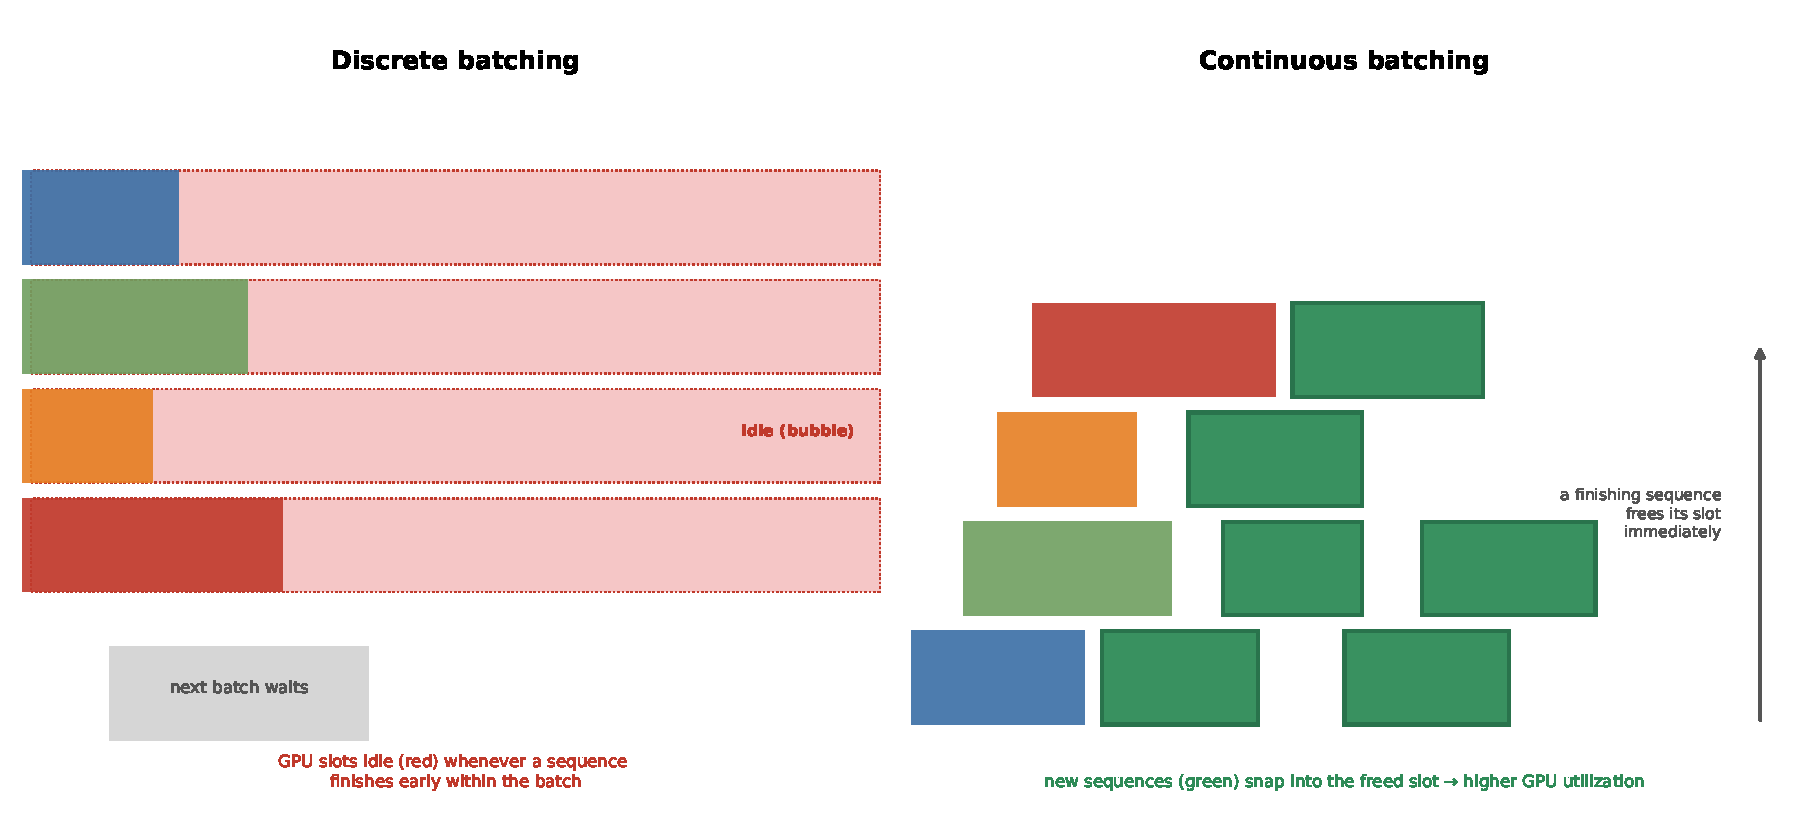
\includegraphics[keepaspectratio,alt={Fig 11.1 --- Discrete vs continuous batching (Orca-style slot diagram). Discrete batching runs each batch to completion, leaving GPU slots idle as sequences finish early; continuous batching admits and evicts requests at every decode step, backfilling freed slots (ILLUSTRATIVE, after Orca, OSDI 2022)},width=\maxwidth{\textwidth},keepaspectratio]{figures/fig-11-1102.pdf}}
\caption{Fig 11.1 --- Discrete vs continuous batching (Orca-style slot
diagram). Discrete batching runs each batch to completion, leaving GPU
slots idle as sequences finish early; continuous batching admits and
evicts requests at every decode step, backfilling freed slots
(ILLUSTRATIVE, after Orca, OSDI 2022)}

\label{fig:11.1}\end{figure}

\emph{\hyperref[fig:11.1]{Fig 11.1} --- The heart of the chapter's serving story made visual.
Discrete (static) batching lets slots sit idle whenever a sequence
finishes early inside the batch; continuous (iteration-level) batching
backfills a freed slot immediately, so the GPU --- not the scheduler ---
is the steady bottleneck. This is the difference between spiky,
latency-wasting batches and a continuously-fed decode pipeline.}

\subsection{PagedAttention: Killing the Fragmentation
Tax}\label{pagedattention-killing-the-fragmentation-tax}

In re-packaged (naive) serving, each request's KV cache for 9.2K input
is \textasciitilde24 GB (FP16, \textasciitilde2.5 MB/token × 9,200)
{[}2° DERIVED{]}. If served contiguously, variable-length completions
leave fragmented, unusable holes --- exactly like a fragmented heap.
\textbf{PagedAttention/vLLM {[}S2{]}{[}1P{]}} allocates KV in fixed
blocks shared and evicted like page frames, so the \textasciitilde24 GB
per request is packed densely and more concurrent requests fit in the
same 640 GB node {[}2° DERIVED{]}. The win is \emph{more concurrency
under the same SLO}, not faster single-request math.

\subsection{Prefix Caching: Don't Re-Prefill the Same
Documents}\label{prefix-caching-dont-re-prefill-the-same-documents}

The RAG request's 8K retrieved-context tokens are largely shared across
queries (same documents). Without caching, every request re-runs the
\textasciitilde1.29 PFLOP prefill for those 8K tokens {[}2° DERIVED{]}.
\textbf{RadixAttention / APC {[}S3{]}{[}1P{]}} caches the KV of common
prefixes, so a new request reuses the shared-document KV and prefills
only the unique query tail --- cutting the dominant prefill FLOPs and
TTFT for repeated-context traffic {[}2° DERIVED{]}.

\subsection{When to Disaggregate: Prefill and Decode Want Different
Pools}\label{when-to-disaggregate-prefill-and-decode-want-different-pools}

Recall from Ch2/Ch6: prefill is \textbf{compute-bound}
(\textasciitilde1.29 PFLOP → \textasciitilde1.19 PFLOPS required vs
0.989 PFLOPS peak), decode is \textbf{bandwidth-bound} (5.6 TB/s demand
vs 3.35 TB/s) {[}2° DERIVED{]}. Serving both from one pool forces a
compromise: batch for prefill and it slows decode; optimize for decode
and prefill starves. \textbf{P/D disaggregation
(Splitwise/DistServe/Mooncake {[}S4{]}{[}1P{]})} runs prefill nodes at
high FLOP-utilization and decode nodes at high bandwidth-utilization,
transferring KV across via the fabric (\textbf{\hyperref[fig:11.3]{Fig 11.3}} shows the
two-pool topology and what moves between them). Mooncake's reported
\textgreater525\% long-context throughput and +75\% request count are
the quantitative anchor {[}S4{]}{[}1P{]}. For the canonical single-host
(\textasciitilde10 rps) this disaggregation is premature; it pays off
only when the workload outgrows a node and the two phases' resource
conflicts become binding.

\subsubsection{\hyperref[tab:11.1]{Table 11-1} --- Serving techniques at a
glance}\label{table-11-1-serving-techniques-at-a-glance}

\begin{longtable}[]{@{}
  >{\raggedright\arraybackslash}p{0.2000\linewidth}
  >{\raggedright\arraybackslash}p{0.2000\linewidth}
  >{\raggedright\arraybackslash}p{0.2000\linewidth}
  >{\raggedright\arraybackslash}p{0.2000\linewidth}
  >{\raggedright\arraybackslash}p{0.2000\linewidth}@{}}
\toprule\noalign{}
\begin{minipage}[b]{\linewidth}\raggedright
Technique
\end{minipage} & \begin{minipage}[b]{\linewidth}\raggedright
Mechanism
\end{minipage} & \begin{minipage}[b]{\linewidth}\raggedright
Primary resource traded
\end{minipage} & \begin{minipage}[b]{\linewidth}\raggedright
When it matters
\end{minipage} & \begin{minipage}[b]{\linewidth}\raggedright
Source
\end{minipage} \\
\midrule\noalign{}
\endhead
\bottomrule\noalign{}
\endlastfoot
Discrete batching & Lock batch to completion & --- (wastes) & baseline
only & {[}1P{]} \\
Continuous batching (Orca) & Admit/evict at each decode step &
compute+bandwidth util & high concurrency & S1 {[}1P{]} \\
PagedAttention / vLLM & Block-based KV pages & memory capacity & many
concurrent requests & S2 {[}1P{]} \\
Prefix caching (RadixAttention/APC) & Cache shared-prefix KV & prefill
FLOPs + memory & repeated-context RAG & S3 {[}1P{]} \\
P/D disaggregation (Splitwise/DistServe/Mooncake) & Split prefill/decode
pools + KV transfer & both at scale & workload outgrows a node & S4
{[}1P{]} \\

\label{tab:11.1}\end{longtable}

\section{Measurement}\label{measurement}

Good serving telemetry answers ``are we meeting the SLO while keeping
the GPU busy?'':

\begin{enumerate}
\def\labelenumi{\arabic{enumi}.}
\item
  \textbf{Measure goodput, not raw throughput} --- tokens/s that arrive
  before their SLO deadline (Ch6). Continuous batching is only a win if
  it raises goodput.
\item
  \textbf{Measure KV utilization} --- fraction of the 640 GB node memory
  consumed by live KV vs weights. PagedAttention and prefix caching both
  raise the effective KV packing; track it.
\item
  \textbf{Measure prefill-vs-decode utilization separately} --- a
  FLOP-bound prefill core and a bandwidth-bound decode core running on
  one pool tells us when to disaggregate.
\item
  \textbf{Measure the scheduler's real occupancy} --- idle decode slots,
  queue wait, and the tail of TTFT under load, not the average.
\end{enumerate}

\section{Common Mistakes}\label{common-mistakes}

\begin{itemize}
\item
  \textbf{Assuming bigger batches always help.} Bigger discrete batches
  raise raw tokens/s but push TTFT past the SLO, zeroing goodput (Ch6).
  Continuous batching exists precisely to uncouple batch size from wait.
\item
  \textbf{Serving KV contiguous and watching fragmentation.}
  PagedAttention removes the fragmentation tax; skipping it wastes
  memory under concurrency.
\item
  \textbf{Re-prefilling shared context.} Without prefix caching,
  repeated RAG documents are recomputed per request --- the single most
  wasteful failure for this workload.
\item
  \textbf{Choosing P/D disaggregation too early.} Splitting pools adds
  fabric + orchestration; for a single host it is overhead without the
  resource conflict that motivates it.
\item
  \textbf{Believing speculative decoding (DFlash \textgreater4.3× / 1.5×
  {[}S5{]}{[}1P{]}) is a serving baseline.} It is an optimization for
  bandwidth-bound decode, not a requirement, and must be validated on
  the workload.
\end{itemize}

\section{Architecture Consequence}\label{architecture-consequence}

The serving stack dictates the deployment choices:

\begin{itemize}
\item
  \textbf{Baseline (canonical single-host):} continuous batching
  (vLLM/Orca) is near-mandatory to hold TTFT under 10 rps input-heavy
  load; PagedAttention ensures the 24 GB-per-request KV pack fits;
  prefix caching is the highest-leverage optimization because the
  workload is repeated-context RAG. This matches the memory and compute
  conclusions of Ch4/Ch7 for the \textasciitilde10 rps \emph{average}
  baseline; at the \textasciitilde40 rps peak the KV budget forces
  replication, which \hyperref[chap:17]{Chapter 17} sizes. {[}S1{]}{[}S2{]}{[}S3{]}{[}1P{]}
\item
  \textbf{Scaling up:} those three carry the workload far before
  disaggregation is justified. FP8 KV (\textasciitilde54\% of BF16
  {[}S6{]}{[}1P{]}) and KV offloading are memory levers available
  without restructuring.
\item
  \textbf{Beyond a node:} when prefill FLOPs and decode bandwidth fight
  on one pool, P/D disaggregation (Splitwise/DistServe/Mooncake) is the
  architecture of choice, with Mooncake's KV-transfer engine moving
  caches between pools. {[}S4{]}{[}1P{]}
\end{itemize}

\begin{figure}
\centering
\pandocbounded{\includegraphics[keepaspectratio,alt={\hyperref[fig:11.2]{Fig 11.2} --- The serving stack: batching, KV management, prefix caching, P/D split {[}ILLUSTRATIVE conceptual{]}},width=\maxwidth{\textwidth},keepaspectratio]{figures/fig-11-1101.pdf}}
\caption{\hyperref[fig:11.2]{Fig 11.2} --- The serving stack: batching, KV management, prefix
caching, P/D split {[}ILLUSTRATIVE conceptual{]}}

\label{fig:11.2}\end{figure}

\emph{\hyperref[fig:11.2]{Fig 11.2} --- From request arrival to token output: continuous
batching, PagedAttention KV, prefix caching, and optional P/D
disaggregation.}

\begin{figure}
\centering
\pandocbounded{\includegraphics[keepaspectratio,alt={\hyperref[fig:11.3]{Fig 11.3} --- P/D disaggregation topology: prefill pool (compute-bound) and decode pool (bandwidth-bound) bridged by KV transfer {[}2° DERIVED{]}},width=\maxwidth{\textwidth},keepaspectratio]{figures/fig-11-1103.pdf}}
\caption{\hyperref[fig:11.3]{Fig 11.3} --- P/D disaggregation topology: prefill pool
(compute-bound) and decode pool (bandwidth-bound) bridged by KV transfer
{[}2° DERIVED{]}}

\label{fig:11.3}\end{figure}

\emph{\hyperref[fig:11.3]{Fig 11.3} --- P/D disaggregation topology. Left: prefill pool,
compute-bound (FLOPs), handles the massive prompt at once. Right: decode
pool, bandwidth-bound (HBM), reads steady token generation. A fabric
bridge moves the per-token KV cache from prefill to decode. The split
exists because the pools want opposite resources --- prefill is
FLOP-starved (\textasciitilde1.19 PFLOPS required vs 0.989 peak), decode
is bandwidth-starved (5.6 TB/s demand vs 3.35 TB/s) {[}2° DERIVED{]}.}

\section{What We Still Don't Know}\label{what-we-still-dont-know}

\begin{itemize}
\tightlist
\item
  \textbf{Portable end-to-end goodput across real enterprise RAG} ---
  Mooncake's 525\%/75\% {[}S4{]}{[}1P{]} and DFlash's 4.3×
  {[}S5{]}{[}1P{]} are strong anchors but are workload-specific; general
  rules are {[}HYPOTHESIS{]}.
\item
  \textbf{Prefix-cache hit rates in mixed traffic} --- the real
  reduction in prefill FLOPs from RadixAttention/APC for a given
  document-distribution is {[}VERIFY{]}.
\item
  \textbf{KV-transfer cost at scale} --- Mooncake's engine moves KV to
  CPU/DRAM/SSD {[}S4{]}{[}1P{]}, but the exact latency/bandwidth
  crossover where disaggregation wins is {[}VERIFY{]}.
\end{itemize}

\section{End-of-Chapter Mini-Case}\label{end-of-chapter-mini-case}

An architect runs the canonical internal Q\&A service on a single 8×H100
host and sees p95 TTFT creep toward 2.2 s against a 2 s SLO as traffic
peaks at 40 rps. Applying this chapter: the architect first confirms
continuous batching is on (vLLM) and that PagedAttention is active ---
otherwise the 24 GB-per-request KV for 9.2K inputs fragments and
concurrency collapses. The biggest lever: prefix caching. The RAG
traffic reuses the same retrieved documents, so the architect enables
automatic prefix caching and watches TTFT drop as the 8K-context prefill
is replaced by cached KV lookups. The architect does \textbf{not} reach
for P/D disaggregation or speculative decoding --- the single host is
resource-sufficient once the wasted re-prefill is eliminated. The
result: p95 TTFT back under 1.8 s at 40 rps, goodput restored, with only
configuration changes --- because the architecture followed the serving
mechanism that matched the workload's repeated-context shape.
